\documentclass[twocolumn]{article}
\usepackage{array,url,kantlipsum}
\usepackage{lmodern}
\usepackage{tikz}
\usepackage{capt-of}
\usepackage{biblatex}
\usepackage{graphicx}
\usepackage{amsmath}
\usepackage{breqn}
\usepackage{rotating}
\usepackage{hyperref}

\usetikzlibrary{arrows,decorations.pathmorphing}

\addbibresource{paperdyna.bib}

\tikzset{>=latex}

\tikzset{snake it/.style={decorate, decoration=snake}}

\newcommand{\Mark}[1]{\textsuperscript{#1}}

\begin{document}
\twocolumn[{%
 \centering
 \LARGE Hybrid ARIMA/ANN vs naive model for trading  \\[1.5em]
 \large Repetto Marco\Mark{1},
       \\[1em]
 \normalsize
 \begin{tabular}{*{2}{>{\centering}p{.35\textwidth}}}
  \Mark{1}Dipartimento di Management e Metodi Quantitativi \tabularnewline
  Università degli studi di Milano \tabularnewline
  \url{}marco.repetto@studenti.unimi.it
 \end{tabular}\\[3em] % some more space after the title part
}]

\begin{abstract}
This paper present the combination of an ARIMA process with the ANN. Such hybrid ARIMA is used for signal generation in the prediction of stock prices movement, especially in such case the goodness of such model is tested in comparison with a naive algorithm that generates signal at random. The portfolio of such game is built using common stocks from NASDAQ and an intraday time series of 90 interval of one minutes each.
\end{abstract}

\section{Introduction}
Trading on securities is probably one of the many field in finance which saw an incredible automatization over recent years and consequently an improvement in efficiency in the markets interested in such innovation\cite{AvellanedaAlgorithmicHighfrequencytrading2011}.

\begin{figure}
    \centering
    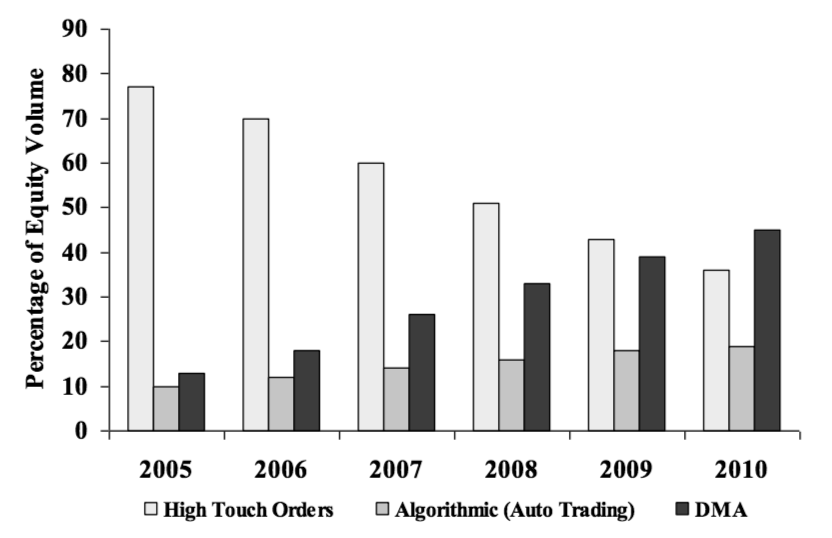
\includegraphics[width=1\linewidth, ]{images/algodata.png}
    \caption{Percentage of order generated by algorithms}
    \label{algodata}
\end{figure}

A completely new professional role came out from such innovation; the Quant, that is, a professional who is expert in quantitative analysis and in particular in financial modelling. The concept of Quant would not be so important without the concept of algorithmic trading, which is defined as automated trading done by computers which are programmed to take certain actions in response to varying market data. In very simplistic and kind of "naive" words the algorithm take the inputs from the model developed by the Quant and enacts the decision supported by the financial model.
In order to let the algorithm implement market decisions (whether to buy or to sell a particular security) we have to "feed" it with a proper financial model. A typical algorithmic trading process is represented on figure \ref{algoproces}; the overall process consists mainly in 4 cyclical phases where two of them interacts comprehend interactions with the environment, as follows:

\begin{itemize}
\item I phase: consists manly on data gathering from the environment $E$, in our case since we are using an univariate time series model our data comes form the sub set $M$ which represent the market data;
\item II phase: at this point the data gathered are used by the Quant to create a proper financial model able to forecast the behaviour of the securities under scope; 
\item III phase: this phase embrace the activities of back-testing of the financial model built by the professional;
\item IV phase: eventually the financial model is deployed and starts to interact with the market $M$, buying and selling a specific security.
\end{itemize}

In this paper we decided to operate a forecast using a model based on time series, precisely an ARIMA (Auto Regressive Integrated Moving Average) process. Plus following what reported by Tseng et al.\cite{zhang_time_2003} we associated to ARIMA process an Artificial Neural Network prepared to capture the behavior of the fitting error of the ARIMA process we built previously. The reason behind this is rather simple, whether the ARIMA process is good at capturing the linear behaviour of our time series this not happens in case of some nonlinearities that may be well fitted by a ANN.
Therefore we defined an algorithm for pseudo real-time signal generation. Based on such signal the algorithm enact the decision whether to buy a stock (forecasting its increase in price) or sell it (because the price will fall). The overall model has to compete with a "naive" algorithm that perform buy and sell decision at random.

\begin{center}
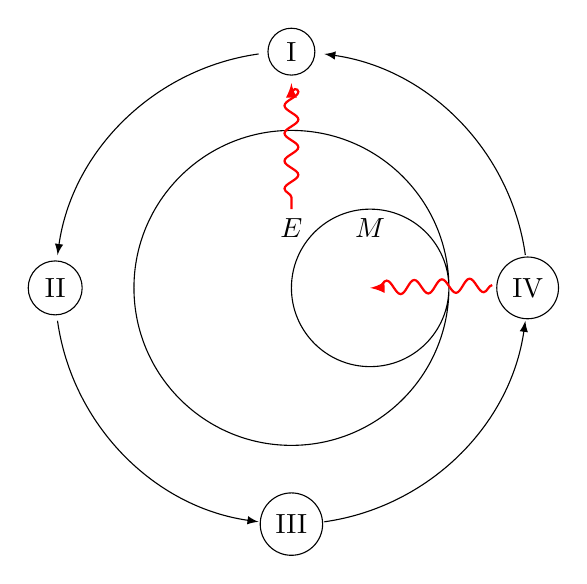
\begin{tikzpicture}

\def \n {4}
\def \radius {3cm}
\def \margin {8} % margin in angles, depends on the radius

  \node[draw, circle] at ({360/\n * (1 - 1)}:\radius) {IV};
  \draw[->, >=latex] ({360/\n * (1 - 1)+\margin}:\radius) 
    arc ({360/\n * (1 - 1)+\margin}:{360/\n * (1)-\margin}:\radius);
    
     \node[draw, circle] at ({360/\n * (2 - 1)}:\radius) {I};
  \draw[->, >=latex] ({360/\n * (2 - 1)+\margin}:\radius) 
    arc ({360/\n * (2 - 1)+\margin}:{360/\n * (2)-\margin}:\radius);
    
     \node[draw, circle] at ({360/\n * (3 - 1)}:\radius) {II};
  \draw[->, >=latex] ({360/\n * (3 - 1)+\margin}:\radius) 
    arc ({360/\n * (3 - 1)+\margin}:{360/\n * (3)-\margin}:\radius);
    
     \node[draw, circle] at ({360/\n * (4 - 1)}:\radius) {III};
  \draw[->, >=latex] ({360/\n * (4 - 1)+\margin}:\radius) 
    arc ({360/\n * (4 - 1)+\margin}:{360/\n * (4)-\margin}:\radius);


\draw (0,0) circle (2) (0,1)  node [text=black,below] {$E$}
      (1,0) circle (1) (1,1)  node [text=black,below] {$M$};
\path [->, thick,draw=red,snake it]
    ({360/5 * (0.9 - 1)+\margin}:2.55) -- (1,0);
\path [<-, thick,draw=red,snake it]
    ({(360/\n * (2 - 1))}:2.6) -- (0,1);
%\draw[draw=blue, snake it] (2,0) arc (0:180:2cm);

\end{tikzpicture}
\end{center}
\captionof{figure}{Algorithmic trading process}
\label{algoproces}
\subsection{AutoRegressive Integrated Moving Average: key concepts and features}
ARIMA process are a class of univariate time series models, this kind of models attempt to predict financial variables using only information contained in their own past values and possibly current and past values of an error term. ARIMA process differ from the exponential smoothing since ARIMA focuses on the autocorrelation of the time series instead of trend and seasonality. Such model firstly proposed by Box-Jenkins\cite{BoxGeorgeTimeSeriesAnalysis} combines three factors, namely: differencing, autoregressive model and moving average model.
\bigbreak
Where differencing is intend as the process of transformation of the time series such that we end up with a stationary time series which has as main property no time dependency, in other terms given $X_t$ a stochastic process and $F_X(x_{t_k+\theta})$ its cumulative distribution. $X_t$ is stationary when; $\forall k,\theta and t_k$ we have that:
\[ F_x(x_{t_{k+\theta}}) = F_x(x_{t_k}) \]
Autoregressive models are instead defined as:
\[ c+\phi_1L+...+\phi_pL^p+\epsilon_t \]
In this models we try to forecast future values using a linear combination of past values.
A different appoach is taken by movin average processes, since they do not use past values but instead a regression of the forecast errors.
Moving average models are defined as:
\[c + (\theta_1 L + ... + \theta_q L^q)\epsilon_t \]
The concatenation of the three gives us the ARIMA process obtained as:

\resizebox{0.90\hsize}{!}{
$
 \underbrace{1-\phi_1L-...-\phi_pL^p}_{AR(p)} + \underbrace{(1-L)^d y_t}_{Differencing(d)} + \underbrace{c + (1 + \theta_1 L + ... + \theta_q L^q)\epsilon_t}_{MA(q)}
$}
In setting such model we used the \textit{forecast} package provided in R \cite{RobHyndmanForecastpackage}
and especially we used the \textit{auto.arima} function to establish 
the proper ARIMA for each time series. The algorithm of choosing the right $(p,d,q)$ coefficients is two-tired \cite{hyndman_automatic_2007}:
\begin{itemize}
    \item Step 1: start with four possible models
\end{itemize} Step 2: consider up to thirteen variations on the current model
When a model score a lower AIC than the current one the new model become the current one and the procedure is repeated until the solution converge to the current model.


\subsection{Artificial Neural Network}
The concept of Artificial Neural Network was firstly proposed by Warren S. McCulloch \cite{mcculloch_logical_1943}.
After a period of stagnation caused by the low processing power of computers at that time, the field saw an incredible expansion in our days and its researching community is one of the most active and perhaps flourish that existed so far.
An Artificial Neural Network is a net based on a series of elements called neurons that are represented by an activation function that given a certain number of input will return an output based on the weights it has.Such activation functions may vary but they are all linear as firstly proposed by B. Widrow \cite{b._widrow_et_al._adaptive_}.
Fundamental for an artificial neural network is the number of hidden layers that compose such network which may vary from 1 to $n$. In our case we used an artificial neural network with just one hidden layer as proposed by the diagram in figure 3.

\tikzset{%
  every neuron/.style={
    circle,
    draw,
    minimum size=0.5cm
  },
  neuron missing/.style={
    draw=none, 
    scale=4,
    text height=0.333cm,
    execute at begin node=\color{black}$\vdots$
  },
}

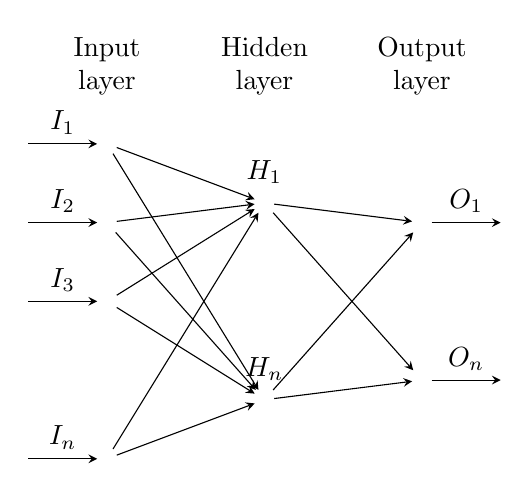
\begin{tikzpicture}[x=1cm, y=1cm, >=stealth]

\foreach \m/\l [count=\y] in {1,2,3,missing,4}
  \node [every neuron/.try, neuron \m/.try] (input-\m) at (0,2.5-\y) {};

\foreach \m [count=\y] in {1,missing,2}
  \node [every neuron/.try, neuron \m/.try ] (hidden-\m) at (2,2-\y*1.25) {};

\foreach \m [count=\y] in {1,missing,2}
  \node [every neuron/.try, neuron \m/.try ] (output-\m) at (4,1.5-\y) {};

\foreach \l [count=\i] in {1,2,3,n}
  \draw [<-] (input-\i) -- ++(-1,0)
    node [above, midway] {$I_\l$};

\foreach \l [count=\i] in {1,n}
  \node [above] at (hidden-\i.north) {$H_\l$};

\foreach \l [count=\i] in {1,n}
  \draw [->] (output-\i) -- ++(1,0)
    node [above, midway] {$O_\l$};

\foreach \i in {1,...,4}
  \foreach \j in {1,...,2}
    \draw [->] (input-\i) -- (hidden-\j);

\foreach \i in {1,...,2}
  \foreach \j in {1,...,2}
    \draw [->] (hidden-\i) -- (output-\j);

\foreach \l [count=\x from 0] in {Input, Hidden, Output}
  \node [align=center, above] at (\x*2,2) {\l \\ layer};

\end{tikzpicture}
\captionof{figure}{Artificial Neural Network scheme}
\label{neural net}

Even though the structure may seem simple one hidden layer ANN reveled to be incredibly reliable on specific task, plus they carry with them greater speed of computation because of its simplicity\cite{the_international_neural_network_society_inns_the_ieee_neural_network_council_cooperating_societies_multi-layer_1990}. As a rule of thumb we take what proposed by Hayashi et al. "Never try a multilayer model for fitting data untill you have tried a single-layer model". Unfortunately there's not such rule of thumb that may help in case of chosing the number of neurons per layer but we choose a number equal two thirds the number of input. 

\subsection{Hybrid ARIMA/ANN process}

The mixed use of ARIMA and neural networks was firstly made by P. Zhang.
Such process compared to the plain vanilla ARIMA has the advantage of capture features that are not modeled by a univariate process like the ARIMA. In our case we use the neural networks to capture the fitting error behavior of the ARIMA process using the lagged stock price of a bucket of randomly picked stock. In this approach we assume that previous price of the portfolio has some kind of relevance of affecting minimally the future price of the stock itself (for example a moment of market bull or bear that affect firstly the other stocks and the the one we modelled).

In theoretical terms we assume a the time series to be constituted by two components one which is linear auto correlated $L_t$ and one $N_t$ non linear. If we let the ARIMA model the linear component we'll end up with the residuals which contains the non linear component.
$$
e_t=y_t-\hat{L_t}
$$
Then we model our residuals with a NN that will capture this non linearities using the normalized stock prices lagged one time.
$$
e_t=f(S^1_{t-1},..., S^k_{t-1})-\epsilon_t
$$

In building an ANN model, subjective judgments of the model order as well as the model adequacy is often needed, and there's no universal rule of thumb on that.Therefore it is possible that sub-optimal models may be used in the hybrid method.

\section{The empirical study}
The empirical study was made using a portfolio built with common stocks from the NASDAQ. Such portfolio was composed by 31 common stocks randomly sampled from the listed company on NASDAQ. From this portfolio we picked each stock and we tested the hybrid ARIMA versus a naive algorithm who generated buy/selling signals at random. We run the game for 30 matches, and every time we retrained our model with the newer information, leaving aside the older ones. The time frame was set at 60 intervals.

\subsection{The 30 stocks portfolio}
In order to get the information of the NASDAQ stock we used the API provided by Alphavantage \cite{_alpha_} and we opted for the 1 minute intraday data from which we took the closing price. In \ref{portfolio} a sample of such dataset.

\begin{figure}
    \centering
    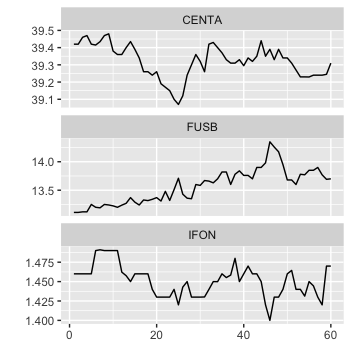
\includegraphics[width=1\linewidth, ]{Paper/images/Rplot.png}
    \caption{Plot of the closing price of some portfolio's stock}
    \label{portfolio}
\end{figure}

From such dataset we run the \textit{auto.arima} function and we isolated the fitting error. %inserire plot

In order to see the goodness of fitting we searched for autocorrelation on the residuals and we found any.

Then we built a NN out of it which set as input the lagged stock price and as output the current error term \ref{NN_plot}.

After the model setting we set a series of condition that create the signal. Such condition are highlighted in the following flowchart.

\begin{tikzpicture}

\end{tikzpicture}


\section{Evidence and findings}
After 930 rounds, that is we run the sequence for all the stocks in the portfolio, we got the following conclusion:
\begin{itemize}
    \item The model out perform the naive algorithm;
    \item The model failed to predict in a consistent way whether the price was going up or down;
    \item Either the models alone failed to do so;
    \item The plain ARIMA performed purely in comparison with the hybrid model.
\end{itemize}

\begin{figure}
    \centering
    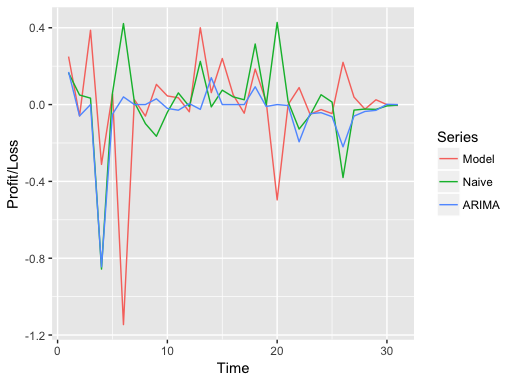
\includegraphics[width=1\linewidth, ]{Paper/images/PL_plot.png}
    \caption{Plot of the aggregate P/L per stock}
    \label{pl_portfolio}
\end{figure}

Therefore we can conclude that such model didn't gave any competitive advantage in terms of profit and loss.

In order to be sure of the forecasting prediction we computed the confusion matrix of each model and we get the following information:
\begin{itemize}
    \item the model out perform the naive algorithm;
    \item the model failed to predict in a consistent way whether the price was going up or down;
    \item either the models alone failed to do so;
    \item the plain ARIMA performed purely in comparison with the hybrid model.
\end{itemize}

\begin{figure}
    \centering
    \includegraphics[width=1\linewidth, ]{Paper/images/.png}
    \caption{Plot of the aggregate P/L per stock}
    \label{pl_portfolio}
\end{figure}

\section{Conclusion}
In conclusion we can say that the hybrid ARIMA however is a very interesting tool for data forecasting is still not able (at least as posed in this paper) to be used in algorithmic trading. 

The writer of this article hope that many other researchers will try to cast some light above this hybrid methodology in order to develop a better process for such modelling.

All the scripts and files are available on GitHub at the following repository:
\href{url}{https://github.com/mrepetto94/DynamicEcon} 

\newpage
\emergencystretch=1em
\sloppy
\printbibliography

\newpage
\newpage

\begin{sidewaysfigure*}[htbp]
\centering
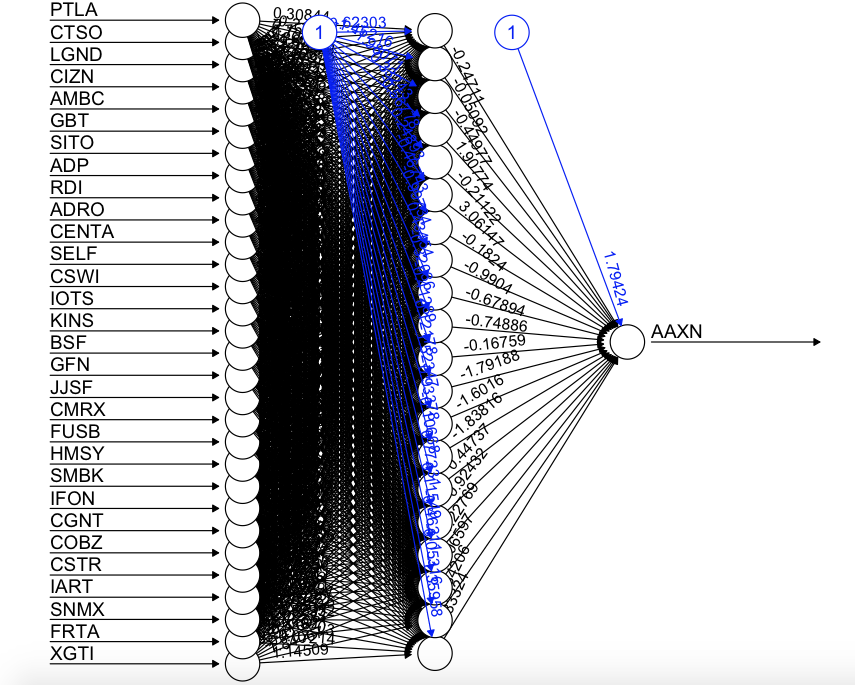
\includegraphics[width=\linewidth, height=\textheight,keepaspectratio]{Paper/images/NN_plot.png}
\caption[short]{\text{Plot of the Neural Network forecasting AAXN current errors}}
\label{NN_plot}
\end{sidewaysfigure*}


\end{document}